% !TEX program = xelatex
% Generated by build_content.py. Actual upstream Metropolis theme, vendored locally.
\documentclass[aspectratio=169,10pt]{beamer}
\usepackage{fontspec,amsmath,amssymb,booktabs,array,tikz,graphicx}
\usetheme[progressbar=frametitle,numbering=fraction,sectionpage=none,block=transparent]{metropolis}
\usetikzlibrary{positioning,arrows.meta}
\setsansfont{FiraSans}[Path=fonts/,Extension=.ttf,UprightFont=*-Regular,BoldFont=*-Bold,ItalicFont=*-Italic]
\setmainfont{FiraSans}[Path=fonts/,Extension=.ttf,UprightFont=*-Regular,BoldFont=*-Bold,ItalicFont=*-Italic]
\setmonofont{Menlo}[Scale=.8]
\definecolor{navy}{HTML}{23373B}
\definecolor{teal}{HTML}{168A85}
\definecolor{blue}{HTML}{2879B8}
\definecolor{purple}{HTML}{8154B8}
\definecolor{muted}{HTML}{68798B}
\definecolor{wash}{HTML}{EFF5F7}
\setbeamerfont{frametitle}{size=\large}
\setbeamerfont{block title}{size=\normalsize,series=\bfseries}
\setbeamerfont{block body}{size=\normalsize}
\setbeamersize{text margin left=.65cm,text margin right=.65cm}
\setlength{\parskip}{.1cm}
\makeatletter
\expandafter\patchcmd\csname beamer@@tmpl@title page\endcsname{\paperheight}{\dimexpr\paperheight-1cm\relax}{}{}
\makeatother
\renewcommand{\arraystretch}{1.12}
\newcolumntype{P}[1]{>{\raggedright\arraybackslash}p{#1}}
\title{Điều khiển đèn giao thông\\từ dữ liệu}
\subtitle{Mô phỏng GAMA và bốn phương pháp điều khiển}
\date{}
\hypersetup{colorlinks=true,urlcolor=blue,linkcolor=teal,pdftitle={Điều khiển đèn giao thông — Seminar}}
\begin{document}

\begin{frame}{A01 · Thứ tự 8 pha được giữ cố định}
\relax

\begin{tabular}{@{}cllc@{}}\toprule
Pha & Trục Bắc–Nam & Trục Đông–Tây & Thời gian\\\midrule
0 & \textcolor{teal}{Xanh đi thẳng} & Đỏ & Thích ứng / 30,1 s cố định\\
1 & Vàng đi thẳng & Đỏ & 3 s\\
2 & \textcolor{blue}{Xanh rẽ trái} & Đỏ & 12 s\\
3 & Vàng rẽ trái & Đỏ & 3 s\\
4 & Đỏ & \textcolor{teal}{Xanh đi thẳng} & Thích ứng / 30,1 s cố định\\
5 & Đỏ & Vàng đi thẳng & 3 s\\
6 & Đỏ & \textcolor{blue}{Xanh rẽ trái} & 12 s\\
7 & Đỏ & Vàng rẽ trái & 3 s\\\bottomrule
\end{tabular}\par
\vspace{.25cm}
\textbf{AI chỉ điều chỉnh pha 0 và 4.} Lịch hiện tại không có pha tất cả đỏ riêng.

\end{frame}
\begin{frame}{A02 · 11 đầu vào của mạng được tạo như thế nào?}
\relax

\begin{tabular}{@{}P{7.2cm}cl@{}}\toprule
Nhóm thông tin & Số chiều & Cách chuẩn hóa\\\midrule
Xe thẳng chờ: B–N, Đ–T & 2 & $\min(n/20,3)$\\
Xe thẳng đang tới: B–N, Đ–T & 2 & $\min(n/20,3)$\\
Xe trái chờ: B–N, Đ–T & 2 & $\min(n/20,3)$\\
Xe phía thoát: B–N, Đ–T & 2 & $\min(n/20,3)$\\
Số bước pha xanh đã qua & 1 & Chia 600\\
Đang pha 0? Đang pha 4? & 2 & Mỗi cờ bằng 0 hoặc 1\\\bottomrule
\end{tabular}\par
\vspace{.3cm}
Ví dụ: 10 xe $\rightarrow$ 0,5; từ 60 xe trở lên $\rightarrow$ 3.\\[.15cm]
\textbf{Chuẩn hóa} giúp đưa các đại lượng về thang số thuận tiện cho mạng.

\end{frame}
\begin{frame}{A03 · Huấn luyện có cải thiện trên validation}
\relax
{\centering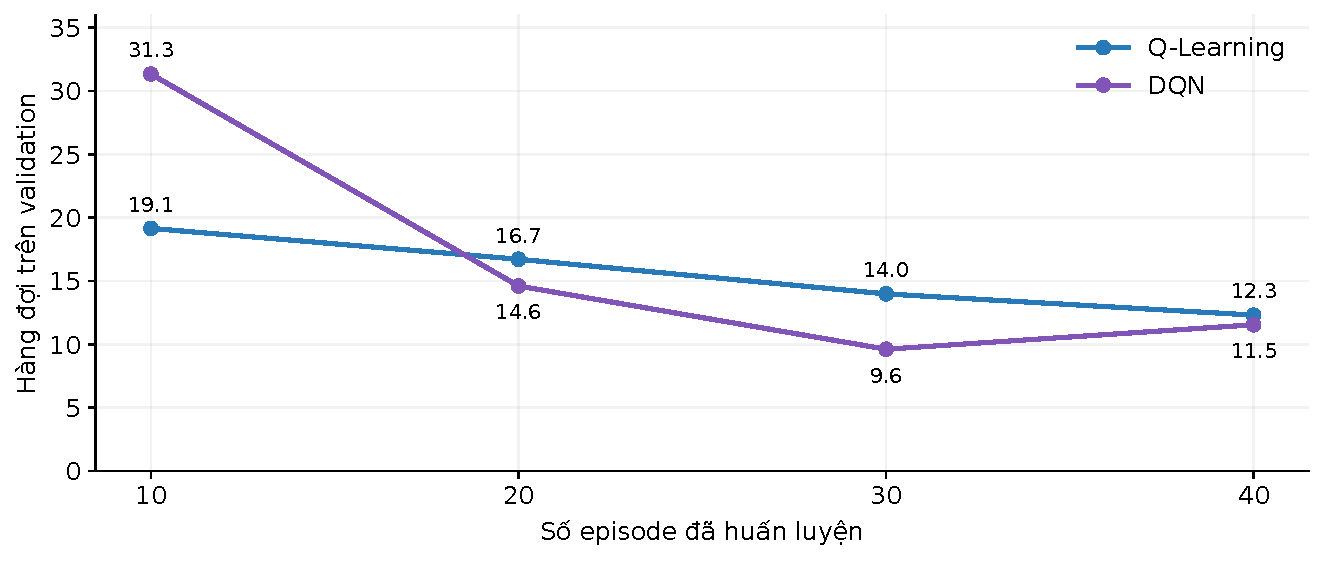
\includegraphics[width=\linewidth,height=4.35cm,keepaspectratio]{figures/validation}\par}\vspace{.15cm}\small Mỗi điểm: trung bình 2 seed validation. Chọn Q ở episode 40; DQN ở episode 30.
\end{frame}
\begin{frame}{A04 · Một phương pháp không thắng ở mọi chỉ số}
\relax

\begin{tabular}{@{}lrrrr@{}}\toprule
Trung bình 5 seed & Fixed & MP & Q & DQN\\\midrule
Xe hoàn thành $\uparrow$ & 228,6 & 232,4 & 238,8 & \textbf{243,6}\\
Hành trình xe xong (s) $\downarrow$ & 277,27 & \textbf{264,64} & 268,83 & 268,23\\
Chờ tích lũy/yêu cầu (s) $\downarrow$ & 292,79 & 289,85 & 287,82 & \textbf{286,97}\\
Chờ ngoài mạng cuối lượt (xe) & 1.045,0 & 1.043,8 & 1.045,4 & 1.044,4\\\bottomrule
\end{tabular}\par
\vspace{.45cm}
\begin{itemize}
\item DQN cao nhất về xe hoàn thành trung bình trong tập này.
\item Max-Pressure thấp nhất về thời gian hành trình của xe đã xong.
\item Chờ/yêu cầu là chi phí đã phát sinh tới horizon; nhiều chuyến chưa kết thúc.
\end{itemize}

\end{frame}
\begin{frame}{A05 · IDM đầy đủ và các đại lượng}
\relax

\[a=a_{\max}\left[1-\left(\frac v{v_0}\right)^\delta-\left(\frac{s^*}{s}\right)^2\right],\quad
s^*=s_0+\max\left(0,vT+\frac{v\Delta v}{2\sqrt{a_{\max}b}}\right)\]
\begin{tabular}{@{}lP{9.3cm}@{}}\toprule
$v,\Delta v$ & Tốc độ xe; tốc độ xe mình trừ tốc độ xe trước (m/s)\\
$s,s_0,s^*$ & Khoảng hở thực; tối thiểu; mong muốn (m)\\
$T$ & Khoảng cách theo thời gian mong muốn (s)\\
$a_{\max},b$ & Tham số tăng tốc và giảm tốc (m/s²)\\
$v_0,\delta$ & Tốc độ đích hiệu dụng; số mũ thành phần đường trống\\\bottomrule\end{tabular}\par
\vspace{.25cm}\small GAMA còn giới hạn tốc độ theo road và \texttt{max\_speed}; dự án có thêm speed cap.

\end{frame}
\begin{frame}{A06 · Cấu hình ba loại xe}
\relax

\begin{tabular}{@{}lrrrrr@{}}\toprule
Loại & Dài (m) & Làn con & $a_{\max}$ & $b$ & $s_0$ (m)\\\midrule
Xe máy & 2,0 & 1 & 2,8 & 4,5 & 0,8\\
Ô tô & 4,6 & 2 & 1,8 & 3,8 & 2,0\\
Buýt & 10,0 & 2 & 1,2 & 2,8 & 3,0\\\bottomrule\end{tabular}\par
\vspace{.4cm}
Tốc độ mong muốn lấy mẫu: xe máy 25–37; ô tô 30–45; buýt 22–32 km/h.\\[.2cm]
Gia tốc/giảm tốc ở bảng dùng m/s².\\[.3cm]
\textbf{Đây là tham số của dự án, chưa phải bảng hiệu chỉnh từ dữ liệu đo.}

\end{frame}
\begin{frame}{A07 · MOBIL và bộ lọc khoảng trống}
\relax

\small
MOBIL kinh điển: lợi ích bản thân + lợi ích xe sau có trọng số phải vượt ngưỡng.
\[\tilde a_c-a_c+p\big[(\tilde a_n-a_n)+(\tilde a_o-a_o)\big]>\Delta a_{\mathrm{th}},\qquad
\tilde a_n\ge-b_{\mathrm{safe}}\]
Dấu $\tilde{\ }$: sau đổi lane; $c$: xe mình; $n/o$: xe sau lane mới/cũ; $p$: mức nhường.
\vspace{.2cm}
\begin{tabular}{@{}lP{8.8cm}@{}}\toprule
Bộ lọc dự án & Điều kiện trước khi cho GAMA xét đổi lane\\\midrule
Có xe cản & Gap $<\max(12\mathrm{m},2\mathrm{s}\cdot v)$; xe trước chậm hơn $>1$ m/s\\
Lane mới, phía trước & Gap $\ge\max(4\mathrm{m},1,5\mathrm{s}\cdot v)$\\
Lane mới, phía sau & Gap $\ge\max(5\mathrm{m},2,5\mathrm{s}(v_{\mathrm{sau}}-v)+5\mathrm{m})$\\\bottomrule\end{tabular}\par
\vspace{.15cm}Các ngưỡng trong bảng là tự đặt; GAMA dùng triển khai lấy cảm hứng từ MOBIL.

\end{frame}
\begin{frame}{A08 · Hình học và luật tốc độ tự triển khai}
\relax

\small
\textbf{Bézier bậc 3:}\quad
$B(t)=(1-t)^3P_0+3(1-t)^2tP_1+3(1-t)t^2P_2+t^3P_3$, $t\in[0,1]$.
\begin{itemize}
\item Dự án lấy 121 điểm để tạo đường; các control point theo hướng vào/ra.
\item Tới cua: $v_{\mathrm{cap}}=\sqrt{v_{\mathrm{cua}}^2+2bd}$ từ động học.
\item Tới vạch dừng: dùng cap bảo thủ với $\sqrt{0,2bg}$ và $g/(4\mathrm{s})$, kèm ramp tốc độ và biên dừng.
\item Theo xe cùng edge: thêm cap dựa trên $\sqrt{v_{\mathrm{trước}}^2+0,5bg}$ và giới hạn thay đổi tốc độ.
\end{itemize}
\begin{block}{Phạm vi nguồn}
Bézier là hình học; quan hệ tốc độ–quãng đường là động học. Hệ số 0,2; 0,5; 4 s và các biên là lựa chọn triển khai, không gán cho IDM/Gipps.
\end{block}

\end{frame}
\begin{frame}{A09 · Trạng thái bảng Q và phạm vi đếm xe}
\relax

\small
\begin{tabular}{@{}P{6.4cm}P{5.8cm}@{}}\toprule
Khóa bảng Q (6 thành phần) & Giá trị\\\midrule
Queue thẳng trục hiện tại / trục kia & Mỗi queue: 0, 1–4, từ 5 trở lên\\
Có xe trái chờ mỗi trục? & Hai cờ 0/1\\
Xe phía thoát trục hiện tại $\ge5$? & Một cờ 0/1\\
Tuổi xanh & $<25$ s; 25–$<45$ s; từ 45 s\\\bottomrule\end{tabular}\par
\vspace{.3cm}
Tối đa $3\times3\times2\times2\times2\times3=216$ khóa, mỗi khóa 2 giá trị Q.\\[.2cm]
DQN dùng vector khác: thêm xe thẳng đang tới và đầu ra của cả hai trục.\\[.2cm]
Phía thoát được lọc theo road mặt đất ra và lane thấp nhất 4–11, không theo danh tính tuyến.

\end{frame}
\begin{frame}{A10 · Loss, gradient và Adam}
\relax

\small
Với $e=Q_\theta(s,a)-y$, Huber (Smooth L1, $\beta=1$):
\[L(e)=\begin{cases}\tfrac12e^2,&|e|<1\\|e|-\tfrac12,&|e|\ge1\end{cases}\]
Loss minibatch là trung bình 64 mẫu. Backpropagation tính $g=\nabla_\theta L$; chuẩn gradient được chặn ở 10.
\[m_t=\beta_1m_{t-1}+(1-\beta_1)g_t,\quad
v_t=\beta_2v_{t-1}+(1-\beta_2)g_t^2\]
\[\hat m_t=\frac{m_t}{1-\beta_1^t},\quad \hat v_t=\frac{v_t}{1-\beta_2^t},\quad
\theta_t=\theta_{t-1}-\eta\frac{\hat m_t}{\sqrt{\hat v_t}+\epsilon_{\mathrm{Adam}}}\]
$\eta=3\times10^{-4}$; $\beta_1=0,9$, $\beta_2=0,999$, $\epsilon_{\mathrm{Adam}}=10^{-8}$ (mặc định PyTorch).\\[.1cm]
$\epsilon_{\mathrm{Adam}}$ chống chia cho 0; khác $\varepsilon$ khám phá.

\end{frame}
\begin{frame}{A11 · Từ điển thuật ngữ để trả lời hỏi đáp}
\relax

\small
\begin{tabular}{@{}P{3.3cm}P{9.1cm}@{}}\toprule
Thuật ngữ & Giải thích\\\midrule
Neuron / lớp ẩn & Phép biến đổi số; không phải xe hay nhánh đường\\
Tensor & Mảng số nhiều chiều PyTorch dùng để tính toán\\
Forward pass & Tính từ đầu vào tới điểm Q bằng trọng số hiện tại\\
Backpropagation & Tính gradient của loss ngược qua các phép biến đổi\\
Learning rate & Mức điều chỉnh tham số trong một update\\
Batch / minibatch & Nhóm mẫu kinh nghiệm dùng chung cho một update\\
Replay buffer & Vùng nhớ lưu transition để lấy mẫu lại\\
Target network & Bản sao thay đổi chậm để tính mục tiêu học\\
Inference & Chọn hành động với mô hình đã có\\
Checkpoint & Gói trạng thái lưu trên đĩa để nạp hoặc tiếp tục học\\\bottomrule\end{tabular}\par

\end{frame}
\begin{frame}{A12 · Nguồn mô hình giao thông}
\relax

\small
\begin{enumerate}
\item[\textbf{[1]}] \href{https://gama-platform.org/wiki/UsingDrivingSkill}{GAMA — Driving Skill}. Saval et al. (2023), \href{https://doi.org/10.1371/journal.pone.0281658}{Dealing with mixed and non-normative traffic}, PLOS ONE.
\item[\textbf{[2]}] Treiber, Hennecke \& Helbing (2000). \href{https://doi.org/10.1103/PhysRevE.62.1805}{Congested traffic states in empirical observations and microscopic simulations}. Physical Review E 62, 1805–1824.
\item[\textbf{[3]}] Kesting, Treiber \& Helbing (2007). \href{https://doi.org/10.3141/1999-10}{General lane-changing model MOBIL for car-following models}. TRR 1999, 86–94.
\item[\textbf{[4]}] Varaiya (2013). \href{https://doi.org/10.1016/j.trc.2013.08.014}{Max pressure control of a network of signalized intersections}. TR Part C 36, 177–195.
\end{enumerate}
\vspace{.25cm}Nguồn thuật toán không tự xác nhận các tỷ lệ xe, ngưỡng lách và hình học riêng của dự án.

\end{frame}
\begin{frame}{A13 · Nguồn học tăng cường và triển khai}
\relax

\small
\begin{enumerate}
\item[\textbf{[5]}] Watkins \& Dayan (1992). \href{https://doi.org/10.1007/BF00992698}{Q-learning}. Machine Learning 8, 279–292.
\item[\textbf{[6]}] Mnih et al. (2015). \href{https://doi.org/10.1038/nature14236}{Human-level control through deep reinforcement learning}. Nature 518, 529–533.
\item[\textbf{[7]}] Bradtke \& Duff. \href{https://proceedings.neurips.cc/paper_files/paper/1994/hash/07871915a8107172b3b5dc15a6574ad3-Abstract.html}{Reinforcement Learning Methods for Continuous-Time Markov Decision Problems}. NIPS 7 (hội nghị 1994, tập in 1995).
\item[\textbf{[8]}] Kingma \& Ba. \href{https://arxiv.org/abs/1412.6980}{Adam: A Method for Stochastic Optimization}. ICLR 2015.
\item[\textbf{[9]}] \href{https://pages.mtu.edu/~shene/COURSES/cs3621/NOTES/spline/Bezier/bezier-construct.html}{Michigan Tech — Bézier curves} (hình học).
\item[\textbf{[10]}] \href{https://docs.pytorch.org/docs/stable/generated/torch.optim.Adam.html}{PyTorch Adam}; \href{https://docs.pytorch.org/docs/stable/generated/torch.nn.SmoothL1Loss.html}{SmoothL1Loss} (triển khai).
\item[\textbf{[11]}] \href{https://openstax.org/books/university-physics-volume-1/pages/3-4-motion-with-constant-acceleration}{OpenStax — Motion with Constant Acceleration}. Cơ sở quan hệ $v^2=u^2+2as$.
\end{enumerate}

\end{frame}
\end{document}
